\section{IIQS exclusive parameters}

In this section we revisit a key parameter of IIQS, the values for $\alpha$ and $\beta$ parameters. As explained previously on Section~\ref{SUBSECTION:IIQS} and in the original work of IIQS~\cite{7416566}, these two values are used during the evaluation of IIQS in order to trigger the execution of a extra partition stage. This extra stage uses a median-of-medians algorithm instead of just relying on the default random pivot selection. The benefit of changing the execution scheme is that it guarantees that the returned median will belong to a position in the central 40 percent of the array.  This extra partition stage has $O(n)$ complexity, hence preserves the original asymptotic bound of the partition algorithm.

\subsection{Understanding median-of-medians usage}
While stated that it does not affect the asymptotic complexity of IQS, it increases its running time by a huge constant factor, as operations performed on BFPRT are not cache friendly for large arrays, specially when implemented in a in-place fashion\footnote{This is because when implemented in-place the idea is not to return the value of the median but rather the index of it. This forces us to move the partial medians generated to a place on which can be cached for next executions and easy controlled. As it is of common knowledge for computer scientists, this position is the beginning of the array.}. 

There is no point on shrinking the \emph{valid area}\footnote{Our central 40\%.} for triggering BFPRT after its evaluation, as there is no guarantee on the resulting distribution of the returned index. Moreover, as BFPRT does not return a median but rather an area on which the median can be found and a partial partitioning of elements~\cite{Blum_Floyd_Pratt_Rivest_Tarjan_1973}, we cannot use this technique as more than a approximate median selection algorithm which shuffles elements along the array.

%% experiment to devise if we can expand the range or we can ignore some bounds.

\begin{figure}[!ht]
    \centering
    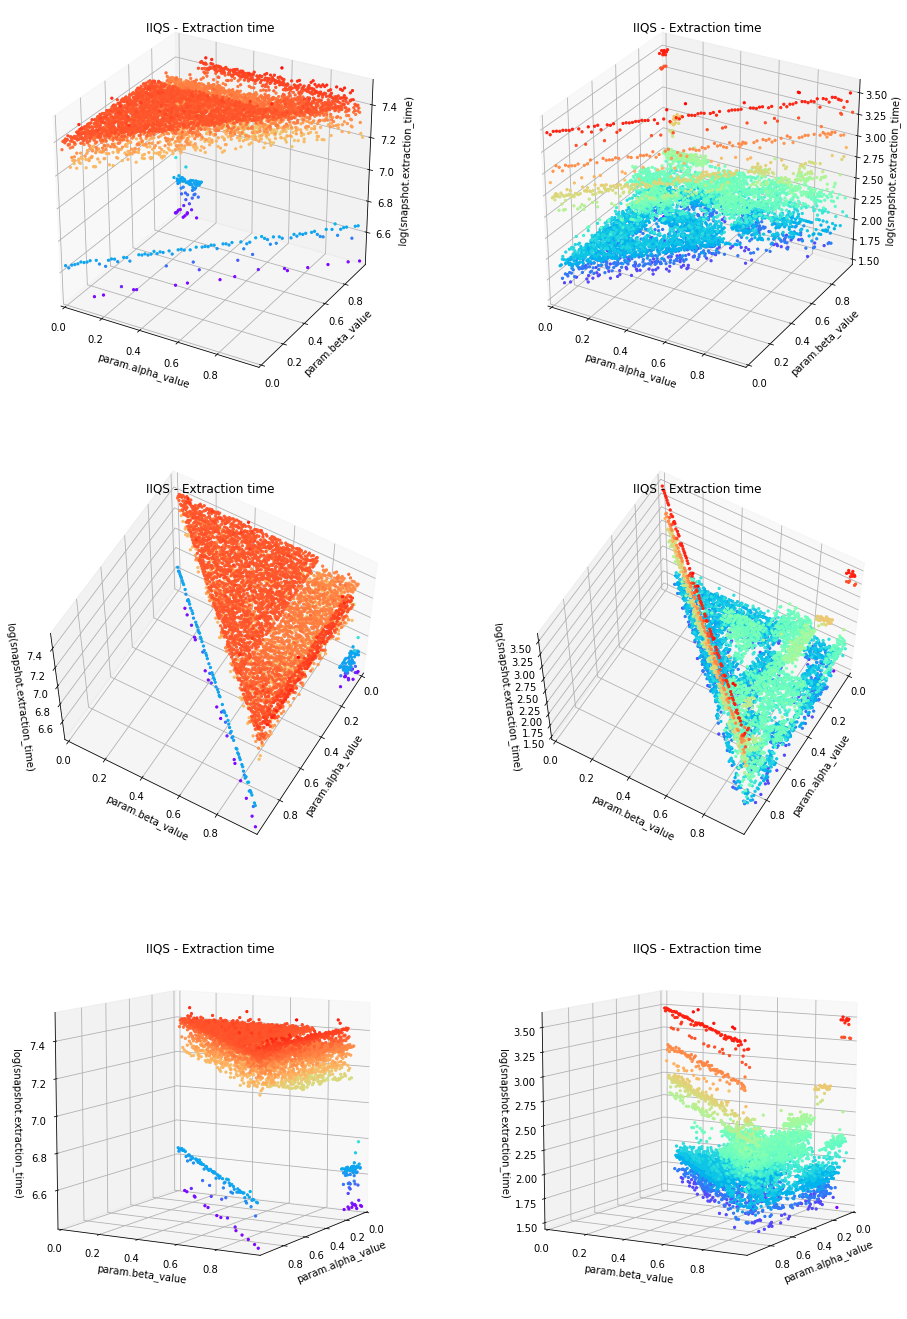
\includegraphics[width=0.8\textwidth]{./fragments/04_experimental_execution/images/04_alphabeta_singleclass.png}
    %\caption{Benchmark for random case. IQS and IIQS executions are shown on the first and second columns respectively.}
    \caption{Benchmark for randomly sorted sequences with$1\times10^5$ unique elements. IIQS executions for the first and second extractions are shown on the first and second column respectively. All extractions using a symlog scale.}
    \label{FIG:05_ALPHABETA_RELATIONSHIP_RANDOM}
\end{figure}

\begin{figure}[!ht]
    \centering
    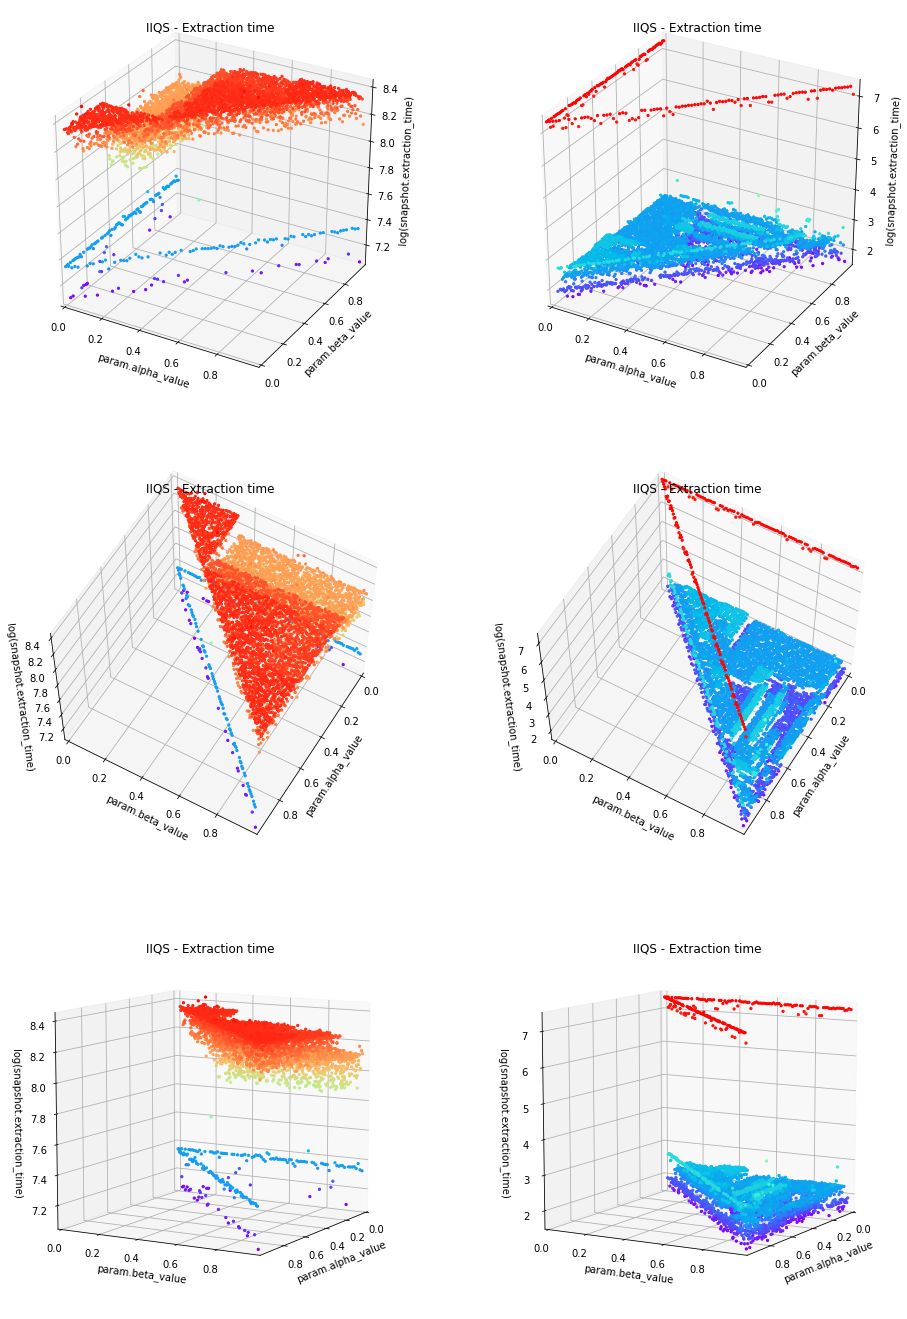
\includegraphics[width=0.8\textwidth]{./fragments/04_experimental_execution/images/04_alphabeta_singleclass_asc.png}
    %\caption{Benchmark for random case. IQS and IIQS executions are shown on the first and second columns respectively.}
    \caption{Benchmark for ascending sequences with$1\times10^5$ unique elements. IIQS executions for the first and second extractions are shown on the first and second column respectively. All extractions using a symlog scale.}
    \label{FIG:05_ALPHABETA_RELATIONSHIP_ASC}
\end{figure}

\begin{figure}[!ht]
    \centering
    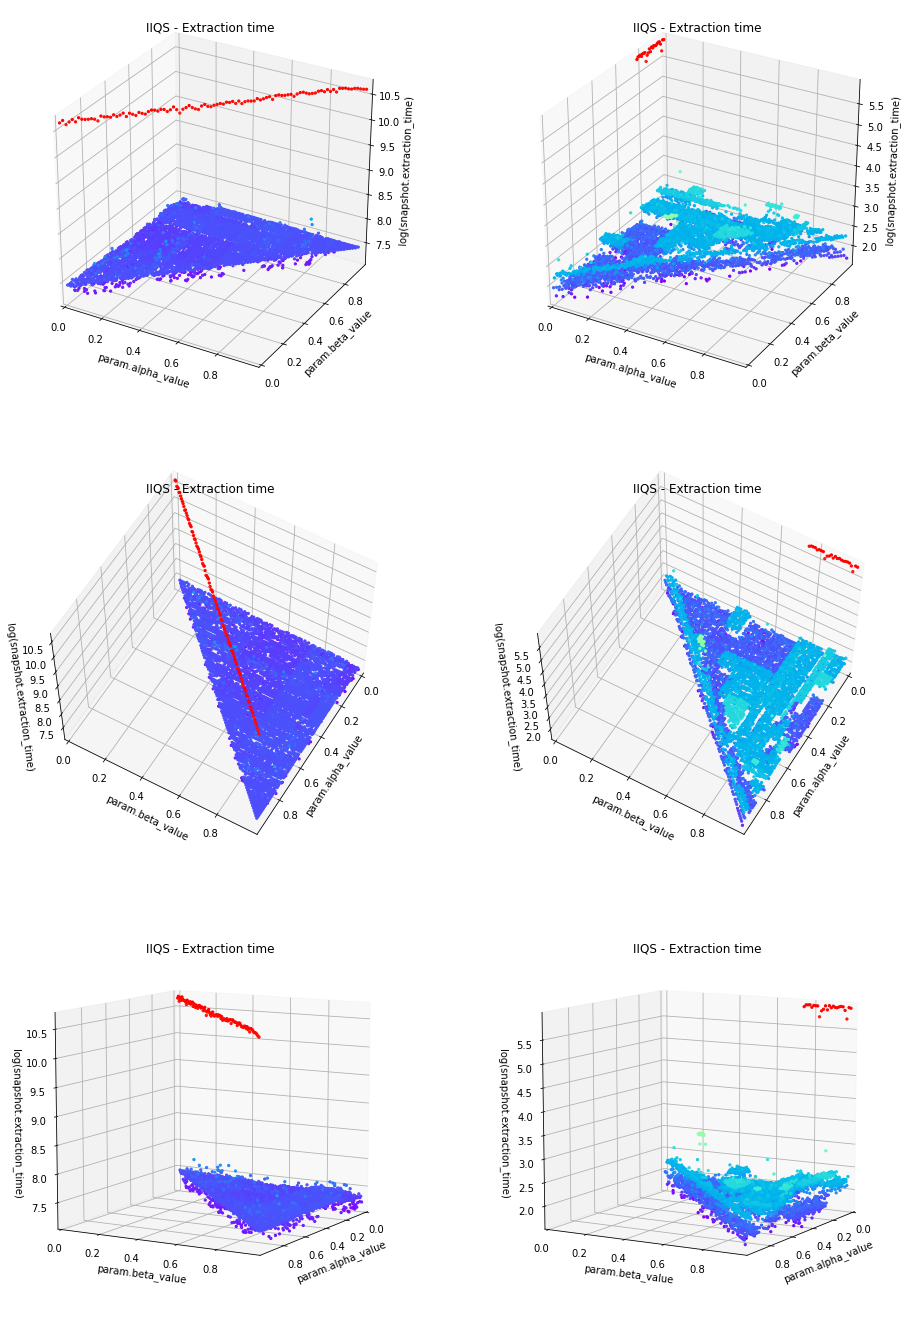
\includegraphics[width=0.8\textwidth]{./fragments/04_experimental_execution/images/04_alphabeta_singleclass_desc.png}
    %\caption{Benchmark for random case. IQS and IIQS executions are shown on the first and second columns respectively.}
    \caption{Benchmark for descending sequences with$1\times10^5$ unique elements. IIQS executions for the first and second extractions are shown on the first and second column respectively. All extractions using a symlog scale.}
    \label{FIG:05_ALPHABETA_RELATIONSHIP_DESC}
\end{figure}


There is a interesting effect resulting of the selection of $\alpha$ and $\beta$ parameters. By just examining the first and second extractions we can appreciate that if we tight the bounds to a point that median-of-medians is executed each time, for all instances we get that the first extraction is accelerated by a huge factor but that comes at a cost of the second extraction being three orders of magnitude larger than the average execution. On the other hand, there are some interesting regions to note. When we start to completely ignore the alpha bound and when beta is lower than $0.5$ there is some noticeable benefit in running time for both instances.

By watching the results of the experiment we clearly identify the following configurations:
\begin{itemize}
    %% list the configurations
\end{itemize}

%% explain why the fuck this is happening
%explaining why that central 40% and why changing that makes you fail


\subsection{Effects of introspective step evaluations}
%lets see what does affect alpha and beta.

